\part{Mathematics}

GNC is applied mathematics. Once you accept this the life will be easier. Once
you made your life easier you can make the decision whether going into applied
mathematics or not. Going into applied mathematics means accepting the
friendship of mathematical rigour. I made this decision and accepted that
mathematics is good and will be part of my life, and I write this book
accordingly.

The mathematics chapter includes a landscape of what mathematics is needed for
GNC in a graph form which is an information retrieval thesaurus. This help you
to see what is the study material and when you feel lost helps you to find the
"You are here!" point on this map.

The interesting part in mathematics comes after calculus. Everything before it
is just dead boring. But, these boring things are the air in the clouds of
Calculus, so that, you have to know these things.

\chapter{The thesaurus of Mathematics}

\begin{tikzpicture}
    [mindmap,
    every node/.style={concept, execute at begin node=\hskip0pt},
    concept color=black!20,
    grow cyclic,
    level 1/.append style={level distance=3cm, sibling angle=30},
    level 2/.append style={level distance=2cm, sibling angle=20}
    ]
    % \clip (-1,2) rectangle ++ (-4,5);
        \node [root concept] {Mathematics} % root
            child { node {Dynamic Systems}
                child { node {Chaos} }
            }
            child { node {Control Theory}
                child { node {Linear systems} }
            }
            child { node {Precalculus 1}
                child { node {Stuff} }
            }
            child { node {Precalculus 2}
                child { node {Stuff} }
            }
            child { node {Precalculus 3}
                child { node {Stuff} }
            }
            % child { node {Precalculus 4}
            %     child { node {Stuff} }
            % }
            ;
\end{tikzpicture}

% \tikz
%   \node {Computational Complexity} % root
%     child { node {Computational Problems}
%       child { node {Problem Measures} }
%       child { node {Problem Aspects} }
%       child { node {Problem Domains} }
%       child { node {Key Problems} }
%     }
%     child { node {Computational Models}
%       child { node {Turing Machines} }
%       child { node {Random-Access Machines} }
%       child { node {Circuits} }
%       child { node {Binary Decision Diagrams} }
%       child { node {Oracle Machines} }
%       child { node {Programming in Logic} }
%     }
%     child { node {Measuring Complexity}
%       child { node {Complexity Measures} }
%       child { node {Classifying Complexity} }
%       child { node {Comparing Complexity} }
%       child { node {Describing Complexity} }
%     }
%     child { node {Solving Problems}
%       child { node {Exact Algorithms} }
%       child { node {Randomization} }
%       child { node {Fixed-Parameter Algorithms} }
%       child { node {Parallel Computation} }
%       child { node {Partial Solutions} }
%       child { node {Approximation} }
%     };


\chapter{Precalculus}
\section{Real Numbers}

\section{Real Numbers - Anki cards}

%ankicard
%ankitags mathematics fundamentals precalculus
%ankifront
\begin{small}
    \begin{tabularx}{1\textwidth}{
            p{\dimexpr1\textwidth\relax}
        }
        \toprule
        \textbf{Real Numbers overview card} \\
        \toprule

        What does the numbers set structure look like? 
        \\
        \midrule

        What are the Natural numbers and its notation?
        \\
        \midrule

        What are the integers and its notation?
        \\
        \midrule

        What are the rational numbers and its notation?
        \\
        \midrule

        What are the irrational numbers and its notation?
        \\
        \midrule

        What are the properties of real numbers? (Commutative, Associative,
        Distributive)
        \\
        \midrule

        What are the rules of Addition and Subtraction?
        \\
        \midrule

        What are the rules of Multiplication and Division?
        \\
        \midrule

        What is the real line and its properties?
        \\
        \midrule

        What are the sets and intervals, its properties, notation and
        operations?
        \\
        \midrule

        What is absolute value and how it relates to distance?
        \\
        \midrule

        What are the properties of absolute value?
        \\
        \bottomrule

    \end{tabularx}
\end{small}
%ankifront end
%ankiback
\begin{small}
    \begin{tabularx}{1\textwidth}{
            p{\dimexpr1\textwidth\relax}
        }
        \toprule
        \textbf{Answers are on the subsequent cards in the topic} \\
        \toprule

    \end{tabularx}
\end{small}
%ankiback end

%ankicard
%ankitags mathematics fundamentals precalculus
\subsection{What does the numbers set structure look like?}
%ankifront
\begin{small}
    \begin{tabularx}{1\textwidth}{
            p{\dimexpr1\textwidth\relax}
        }
        \toprule
        \textbf{What does the numbers set structure look like?}\\
        \bottomrule

    \end{tabularx}
\end{small}
%ankifront end
%ankiback
\begin{small}
    \begin{tabularx}{1\textwidth}{
            p{\dimexpr1\textwidth\relax}
        }
        \toprule
        \textbf{The numbers set  structure looks like the following:} \\
        \midrule

        \makecell{
            Real numbers set, notation: $\mathbb{R}$, includes:\\
            Rational numbers, Notation: $ \mathbb{Q}; \text{ example: } \frac{4}{3}, 9.324$\\
            Irrational numbers, Notation: $ \mathbb{I}; \text{ example: } \sqrt{2} \pi $\\
            \\ 
            Rational numbers set includes:\\
            Integers, Notation: $\mathbb{Z} \text{ example: } -1, 2, 3, \cdots $\\
            \\
            Integers number set includes:\\
            Natural numbers, Notation: $\mathbb{N}, \text{ example: } 1, 2, 3 \cdots$
        }
        \\
        \bottomrule

    \end{tabularx}
\end{small}
%ankiback end

%ankicard
%ankitags mathematics fundamentals precalculus
\subsection{What are the Natural numbers and its notation?}
%ankifront
\begin{small}
    \begin{tabularx}{1\textwidth}{
            p{\dimexpr1\textwidth\relax}
        }
        \toprule
        What are the Natural numbers and its notation?
        \\
        \bottomrule

    \end{tabularx}
\end{small}
%ankifront end
%ankiback
\begin{small}
    \begin{tabularx}{1\textwidth}{
            p{\dimexpr1\textwidth\relax}
        }
        \toprule
            Natural numbers, Notation: $\mathbb{N}, \text{ example: } 1, 2, 3 \cdots$\\
        \bottomrule

    \end{tabularx}
\end{small}
%ankiback end

%ankicard
%ankitags mathematics fundamentals precalculus
\subsection{What are the Integers and its notation?}
%ankifront
\begin{small}
    \begin{tabularx}{1\textwidth}{
            p{\dimexpr1\textwidth\relax}
        }
        \toprule
        What are the integers and its notation?
        \\
        \bottomrule

    \end{tabularx}
\end{small}
%ankifront end
%ankiback
\begin{small}
    \begin{tabularx}{1\textwidth}{
            p{\dimexpr1\textwidth\relax}
        }
        \toprule
            Integers, Notation: $\mathbb{Z} \text{ example: } -1, 2, 3, \cdots $\\

    \end{tabularx}
\end{small}
%ankiback end

%ankicard
%ankitags mathematics fundamentals precalculus
\subsection{What are the Rational numbers and its notation?}
%ankifront
\begin{small}
    \begin{tabularx}{1\textwidth}{
            p{\dimexpr1\textwidth\relax}
        }
        \toprule
        What are the rational numbers and its notation?
        \\
        \bottomrule

    \end{tabularx}
\end{small}
%ankifront end
%ankiback
\begin{small}
    \begin{tabularx}{1\textwidth}{
            p{\dimexpr1\textwidth\relax}
        }
        \toprule
        Rational numbers, Notation: $ \mathbb{Q}; \text{ example: } \frac{4}{3}, 9.324$\\
        \bottomrule

    \end{tabularx}
\end{small}
%ankiback end

%ankicard
%ankitags mathematics fundamentals precalculus
\subsection{What are the Irrational numbers and its notation?}
%ankifront
\begin{small}
    \begin{tabularx}{1\textwidth}{
            p{\dimexpr1\textwidth\relax}
        }
        \toprule
        What are the irrational numbers and its notation?
        \\
        \bottomrule

    \end{tabularx}
\end{small}
%ankifront end
%ankiback
\begin{small}
    \begin{tabularx}{1\textwidth}{
            p{\dimexpr1\textwidth\relax}
        }
        \toprule
        Irrational numbers, Notation: $ \mathbb{I}; \text{ example: } \sqrt{2}, \pi $\\
        \bottomrule

    \end{tabularx}
\end{small}
%ankiback end

%ankicard
\subsection{What are the properties of Real Numbers?}

\begin{tabularx}{1\textwidth}{
    p{\dimexpr0.5\textwidth\relax}
    p{\dimexpr0.5\textwidth\relax}
}
\toprule
\multicolumn{2}{c}{\textbf{Properties of real numbers}} \\
\midrule

\textbf{Property} & \textbf{Example}\\
\midrule

\makecell[l]{
    \textbf{Commutative Properties} \\ 1[ex]
    $a + b = b + a$ \\ 
    $a \cdot b = b \cdot a$
} 
& 
\makecell[l]{
    $4 + 3 = 3 + 4$ \\ 
    $4 \cdot 3 = 3 \cdot 4$
} 
\\
\midrule

\makecell[l]{
    \textbf{Associative Properties} \\[1ex] 
    $(a + b) + c = a + (b + c)$ \\ 
    $(a \cdot b) \cdot c = a \cdot (b \cdot c)$
} 
&
\makecell[l]{
    $(2 + 3) + 4 = 2 + (3 + 4)$ \\ 
    $(2 \cdot 3) \cdot 4 = (2 \cdot 3) \cdot 4$
} 
\\

\midrule

\makecell[l]{
    \textbf{Distributive Properties} \\[1ex] 
    $a(b + c) = a \cdot b + a \cdot c$ \\ 
    $(b + c) \cdot a = a \cdot b + a \cdot c$
} 
& 
\makecell[l]{
    $2(3 + 4) = 2 \cdot 3 + 2 \cdot 4$ \\ 
    $(3 + 4) \cdot 2 = 3 \cdot 2 + 4 \cdot 2$
} 
\\  

\bottomrule
\end{tabularx}
%ankicard end

%ankicard
%ankitags mathematics algebra precalculus
\subsection{What are the properties of Addition and Subtraction?}

\begin{tabularx}{1\textwidth}{
    p{\dimexpr0.5\textwidth\relax}
    p{\dimexpr0.5\textwidth\relax}
}
\toprule
\multicolumn{2}{c}{\textbf{Rules of Addition and Subtraction}} \\
\midrule

\textbf{Property} & \textbf{Example}\\
\midrule

\makecell[l]{
    $(-1)a = -a$
} 
& 
\makecell[l]{
    $(-1)5 = -5$
} 
\\
\makecell[l]{
    $-(-a) = a$
} 
& 
\makecell[l]{
    $-(-5) = 5$
} 
\\
\makecell[l]{
    $(-a)b = a(-b) = -(ab)$
} 
& 
\makecell[l]{
    $(-3)5 = 5(-3) = -(5 \cdot 3)$
} 
\\
\makecell[l]{
    $(-a)(-b) = ab$
} 
& 
\makecell[l]{
    $(-3)(-5) = 5 \cdot 3$
} 
\\
\makecell[l]{
    $-(a+b) = -a-b$
} 
& 
\makecell[l]{
    $-(3+5) = -5-3$
} 
\\
\makecell[l]{
    $-(a-b) = b-a = -a + b$
} 
& 
\makecell[l]{
    $-(3-5) = 5-3 = -3+5$
} 
\\

\bottomrule
\end{tabularx}
%ankicard end

%ankicard
%ankitags mathematics algebra precalculus
\subsection{What are the properties of Multiplication and Division?}

%ankifront
\begin{small}
    \begin{tabularx}{1\textwidth}{
        p{\dimexpr1\textwidth\relax}
    }
        \toprule
        \textbf{What are the Rules of Multiplication and Division?} \\
        \midrule
    \end{tabularx}
\end{small}
%ankifront end

%ankiback
\begin{small}
    \begin{tabularx}{1\textwidth}{
            p{\dimexpr1\textwidth\relax}
        }

        \textbf{Properties of Multiplication and Division} \\
    \midrule

    \makecell[l]{
        \vspace{5pt}
        1, $ \frac{a}{b} \cdot \frac{c}{d} = \frac{ac}{bd} $
        \vspace{5pt}
    } 
    \\
    \makecell[l]{
        \vspace{5pt}
    2, $ \frac{a}{b} \div \frac{c}{d} = \frac{a}{b} \cdot \frac{d}{c} $
        \vspace{5pt}
    } 
    \\
    \makecell[l]{
        \vspace{5pt}
    3, $ \frac{a}{c} + \frac{b}{c} = \frac{a + b}{c} $
        \vspace{5pt}
    } 
    \\
    \makecell[l]{
        \vspace{5pt}
    4, $ \frac{a}{b} + \frac{c}{d} = \frac{ad + cb}{bd} $
        \vspace{5pt}
    } 
    \\
    \makecell[l]{
        \vspace{5pt}
        5,  $ \frac{ac}{bc} = \frac{a}{b} $
        \vspace{5pt}
    } 
    \\
    \makecell[l]{
        \vspace{5pt}
    6, $ \text{If } \frac{a}{b} = \frac{c}{d}, \text{then } ad = bc$
        \vspace{5pt}
    } 
    \\
    \bottomrule
    \end{tabularx}
\end{small}
%ankiback end

%ankicard
\subsection{The Real Line}

The properties of the Real Line:

\begin{itemize}
    \item reference point is called origin, its value is $0$
    \item each positive $x$ number is represented on the right side
    \item each negative $-x$ number is represented on the left side
    \item the number assiciated with the point $P$ is called the coordinate of
        $P$
    \item the real numbers are ordered:
    \begin{itemize}
        \item $a$ is less than $b$,  $a < b$ if $b - a$ is a positive number,
            meaning $a$ lies on the left of $b$ on the number line
        \item $a$ is greater than $b$, $a > b$ when $a - b$ is a negative
            number, meaning $a$ lies on the right side of $b$ on the number line
    \end{itemize}
\end{itemize}
%ankicard end

%ankicard
\subsection{Sets and Intervals}

A \textbf{Set} is a collection of objects called \textbf{elements}.

Notation:
\begin{itemize}
    \item $S$ is a set
    \item $a \in S$ means $a$ is element of $S$
    \item $b \notin S$ means $b$ is not element of $S$
    \item $S$ and $T$ are sets and their union is $S \cup T$ and consists all of
        elements that either member of $S$ or $T$ or both
    \item the intersection of $S \cap T$ means the elements part of both sets, in
        other words, this is the common part of both sets
    \item the empty set is denoted by $\emptyset$
\end{itemize}

The listing the elements notation of a set:

\begin{center}
$A = \{1, 2, 3, 4, 5\}$
\end{center}

The builder notion of a set: 

\begin{center}
$ A = \{x | x \text{ is an integer and } 0 < x < 8 \}$
\end{center}
%ankicard end

%ankicard
%ankitags mathematics algebra precalculus
\subsection{What are the notations of intervals?}
%ankifront

\begin{small}
    \begin{tabularx}{1\textwidth}{
        p{\dimexpr1\textwidth\relax}
    }
    \toprule
    \textbf{What are the notations of intervals?} \\
    \bottomrule
    \end{tabularx}
\end{small}
%ankifront end
%ankiback

\begin{small}
\begin{tabularx}{1\textwidth}{
    p{\dimexpr0.3\textwidth\relax}
    p{\dimexpr0.3\textwidth\relax}
    p{\dimexpr0.4\textwidth\relax}
}
\toprule
Notation & Set Description & Graph \\
\midrule

$ \left( a,b \right) $ &
$ \left\{ x | a < x < b \right\} $ &
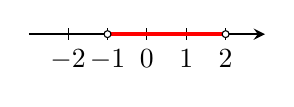
\begin{tikzpicture}[scale=0.5]
  % Drawing the real number line
  \draw[thick, -stealth] (-3,0) -- (3,0); % Main line with arrow
  \foreach \x in {-2,-1,0,1,2} {
    \draw (\x,0.15) -- (\x,-0.15) node[below] {$\x$}; % Tick marks and labels
  }
  % \draw (0,0.3) -- (0,-0.3) node[below] {$0$}; % Emphasize origin

  % Marking the interval [-2, 3)
  \draw[line width=1.5pt, red] (-1,0) -- (2,0); % Thick line for interval
  \draw[black, fill=white] (-1,0) circle (2.5pt); % Closed endpoint at -2
  \draw[black, fill=white] (2,0) circle (2.5pt); % Open endpoint at 3
\end{tikzpicture}
\\
\midrule

$ \lbrack a,b \rbrack $ &
$ \left\{ x | a \leq x \leq b \right\} $ &
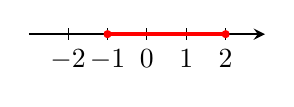
\begin{tikzpicture}[scale=0.5]
  % Drawing the real number line
  \draw[thick, -stealth] (-3,0) -- (3,0); % Main line with arrow
  \foreach \x in {-2,-1,0,1,2} {
    \draw (\x,0.15) -- (\x,-0.15) node[below] {$\x$}; % Tick marks and labels
  }
  % \draw (0,0.3) -- (0,-0.3) node[below] {$0$}; % Emphasize origin

  % Marking the interval [-2, 3)
  \draw[line width=1.5pt, red] (-1,0) -- (2,0); % Thick line for interval
  \filldraw[red] (-1,0) circle (2.5pt); % Closed endpoint at -2
  \filldraw[red] (2,0) circle (2.5pt); % Open endpoint at 3
\end{tikzpicture}
\\
\midrule

$ \lbrack a,b ) $ &
$ \left\{ x | a \leq x < b \right\} $ &
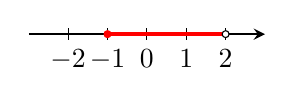
\begin{tikzpicture}[scale=0.5]
  % Drawing the real number line
  \draw[thick, -stealth] (-3,0) -- (3,0); % Main line with arrow
  \foreach \x in {-2,-1,0,1,2} {
    \draw (\x,0.15) -- (\x,-0.15) node[below] {$\x$}; % Tick marks and labels
  }
  % \draw (0,0.3) -- (0,-0.3) node[below] {$0$}; % Emphasize origin

  % Marking the interval [-2, 3)
  \draw[line width=1.5pt, red] (-1,0) -- (2,0); % Thick line for interval
  \filldraw[red] (-1,0) circle (2.5pt); % Closed endpoint at -2
  \draw[black, fill=white] (2,0) circle (2.5pt); % Open endpoint at 3
\end{tikzpicture}
\\

\midrule
$ ( a,b \rbrack $ &
$ \left\{ x | a < x \leq b \right\} $ &
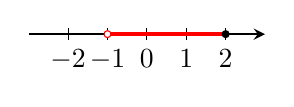
\begin{tikzpicture}[scale=0.5]
  % Drawing the real number line
  \draw[thick, -stealth] (-3,0) -- (3,0); % Main line with arrow
  \foreach \x in {-2,-1,0,1,2} {
    \draw (\x,0.15) -- (\x,-0.15) node[below] {$\x$}; % Tick marks and labels
  }
  % \draw (0,0.3) -- (0,-0.3) node[below] {$0$}; % Emphasize origin

  % Marking the interval [-2, 3)
  \draw[line width=1.5pt, red] (-1,0) -- (2,0); % Thick line for interval
  \draw[red, fill=white] (-1,0) circle (2.5pt); % Closed endpoint at -2
  \filldraw[black] (2,0) circle (2.5pt); % Open endpoint at 3
\end{tikzpicture}
\\
\midrule

$ ( a,\infty ) $ &
$ \left\{ x | a < \infty \right\} $ &
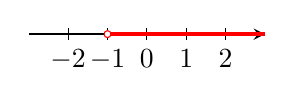
\begin{tikzpicture}[scale=0.5]
  % Drawing the real number line
  \draw[thick, -stealth] (-3,0) -- (3,0); % Main line with arrow
  \foreach \x in {-2,-1,0,1,2} {
    \draw (\x,0.15) -- (\x,-0.15) node[below] {$\x$}; % Tick marks and labels
  }
  % \draw (0,0.3) -- (0,-0.3) node[below] {$0$}; % Emphasize origin

  % Marking the interval [-2, 3)
  \draw[line width=1.5pt, red] (-1,0) -- (3,0); % Thick line for interval
  \draw[red, fill=white] (-1,0) circle (2.5pt); % Closed endpoint at -2
  % \filldraw[black] (2,0) circle (2.5pt); % Open endpoint at 3
\end{tikzpicture}
\\
\midrule

$ \lbrack a,\infty ) $ &
$ \left\{ x | a \leq \infty \right\} $ &
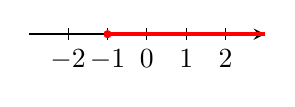
\begin{tikzpicture}[scale=0.5]
  % Drawing the real number line
  \draw[thick, -stealth] (-3,0) -- (3,0); % Main line with arrow
  \foreach \x in {-2,-1,0,1,2} {
    \draw (\x,0.15) -- (\x,-0.15) node[below] {$\x$}; % Tick marks and labels
  }
  % \draw (0,0.3) -- (0,-0.3) node[below] {$0$}; % Emphasize origin

  % Marking the interval [-2, 3)
  \draw[line width=1.5pt, red] (-1,0) -- (3,0); % Thick line for interval
  \filldraw[red] (-1,0) circle (2.5pt); % Closed endpoint at -2
  % \filldraw[black] (2,0) circle (2.5pt); % Open endpoint at 3
\end{tikzpicture}
\\
\midrule

$ ( -\infty, a ) $ &
$ \left\{ x | x < a \right\} $ &
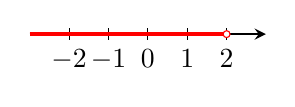
\begin{tikzpicture}[scale=0.5]
  % Drawing the real number line
  \draw[thick, -stealth] (-3,0) -- (3,0); % Main line with arrow
  \foreach \x in {-2,-1,0,1,2} {
    \draw (\x,0.15) -- (\x,-0.15) node[below] {$\x$}; % Tick marks and labels
  }
  % \draw (0,0.3) -- (0,-0.3) node[below] {$0$}; % Emphasize origin

  % Marking the interval [-2, 3)
  \draw[line width=1.5pt, red] (-3,0) -- (2,0); % Thick line for interval
  \draw[red, fill=white] (2,0) circle (2.5pt); % Closed endpoint at -2
  % \filldraw[black] (2,0) circle (2.5pt); % Open endpoint at 3
\end{tikzpicture}
\\
\midrule

$ ( -\infty, a \rbrack $ &
$ \left\{ x | x \leq a \right\} $ &
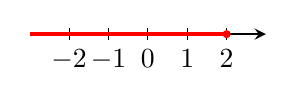
\begin{tikzpicture}[scale=0.5]
  % Drawing the real number line
  \draw[thick, -stealth] (-3,0) -- (3,0); % Main line with arrow
  \foreach \x in {-2,-1,0,1,2} {
    \draw (\x,0.15) -- (\x,-0.15) node[below] {$\x$}; % Tick marks and labels
  }
  % \draw (0,0.3) -- (0,-0.3) node[below] {$0$}; % Emphasize origin

  % Marking the interval [-2, 3)
  \draw[line width=1.5pt, red] (-3,0) -- (2,0); % Thick line for interval
  \filldraw[red] (2,0) circle (2.5pt); % Closed endpoint at -2
  % \filldraw[black] (2,0) circle (2.5pt); % Open endpoint at 3
\end{tikzpicture}
\\
\midrule

$ ( -\infty, \infty ) $ &
$ \mathbb{R} \text{set of real numbers} $ &
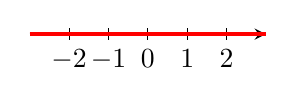
\begin{tikzpicture}[scale=0.5]
  % Drawing the real number line
  \draw[thick, -stealth] (-3,0) -- (3,0); % Main line with arrow
  \foreach \x in {-2,-1,0,1,2} {
    \draw (\x,0.15) -- (\x,-0.15) node[below] {$\x$}; % Tick marks and labels
  }
  % \draw (0,0.3) -- (0,-0.3) node[below] {$0$}; % Emphasize origin

  % Marking the interval [-2, 3)
  \draw[line width=1.5pt, red] (-3,0) -- (3,0); % Thick line for interval
  % \filldraw[red] (2,0) circle (2.5pt); % Closed endpoint at -2
  % \filldraw[black] (2,0) circle (2.5pt); % Open endpoint at 3
\end{tikzpicture}
\\
\midrule

\end{tabularx}
\end{small}
%ankiback end

%ankicards
%ankitags mathematics algebra precalculus

\subsection{What are the rules of Absolute Value?}

\begin{small}
\begin{tabularx}{1\textwidth}{
    p{\dimexpr0.4\textwidth\relax}
    p{\dimexpr0.6\textwidth\relax}
}
\toprule
Rule & Description \\
\midrule

\[ 
    \lvert a \rvert =  
    \begin{cases}
        a  & \text{ if } a \geq 0 \\
        -a & \text{ if } a < 0
    \end{cases}
\] 
&  
when $a$ is a real number 
\\
\midrule

$ \lvert a \rvert \geq 0 $
&
The absolute value of a number is always positive or zero
\\
\midrule

$ \lvert a \rvert = \lvert -a \rvert $
&
A number and its negative have the same absolute value
\\
\midrule

$ \lvert ab \rvert = \lvert a \rvert \lvert b \rvert $
&
The absolute value of a product is the product of the absolute values
\\
\midrule

$ \lvert \frac{a}{b} \rvert = \frac{\lvert a \rvert}{\lvert b \rvert} $
&
The absolute value of a quotient is the quotient of the absolute values
\\
\midrule

$ \lvert a + b \rvert = \lvert a \rvert + \lvert b \rvert $
&
Triangle Inequality
\\

\bottomrule

\end{tabularx}
\end{small}

%ankicards end

%ankicard
%ankitags mathematics algebra precalculus
\subsection{Distance of two points on the Real Line}
%ankifront
\begin{small}
    \begin{tabularx}{1\textwidth}{
            p{\dimexpr1\textwidth\relax}
        }
        \toprule
        \textbf{Distance of two points on the Real Line} \\
        \bottomrule
    \end{tabularx}
\end{small}
%ankifront end

%ankiback

% \begin{small}
\begin{tabularx}{1\textwidth}{
        p{\dimexpr0.5\textwidth\relax}
        p{\dimexpr0.5\textwidth\relax}
    }
\toprule
\multicolumn{2}{c}{\textbf{Distance between two points}} \\
\midrule

$ d(a, b) = \left| b - a \right| $ &
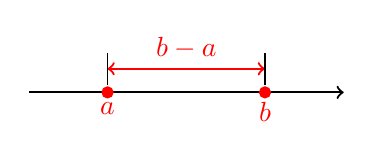
\begin{tikzpicture}
    % Draw the line
    \draw[thick, ->] (0,0) -- (4,0);
    
    % Draw points
    \filldraw[red] (1,0) circle (2pt) node[below] {$a$};
    \filldraw[red] (3,0) circle (2pt) node[below] {$b$};
    
    % Draw the vector
    \draw[red, thick, <->] (1,0.3) -- (3,0.3) node[midway, above] {$ \lvert b - a \rvert $};
    \draw[black] (1,0.1) -- ++(0,0.4);
    \draw[black] (3,0.1) -- ++(0,0.4);
    % \draw[red, thick, <-] (0,-0.2) -- (4,-0.2);
\end{tikzpicture}
\\
\bottomrule


\end{tabularx}
% \end{small}
%ankiback end


\section{Exponents}

\section{Exponents - Anki cards}

\section{Exponents}

\section{Exponents - Anki cards}

\section{Exponents}

\section{Exponents - Anki cards}

\input{mathematics/algebra/exponents/ankicards/exponents}



%ankicard
\subsection{What are the Laws of Roots?}

$$
\sqrt[n]{ab} = \sqrt[n]{a} \cdot \sqrt[n]{b} 
$$

$$
\sqrt[n]{ \frac{a}{b} } = \frac{ \sqrt[n]{a} }{ \sqrt[n]{a} }
$$

$$
\sqrt[n]{ \sqrt[m]{a}} = \sqrt[n \cdot m]{a} 
$$

$$
\sqrt[n]{ a^{n} } = a, \text{ if } n \text{ odd }
$$
$$ 
\sqrt[n]{ a^{n} } = \lvert a \rvert, \text{ if } n \text{ is even }
$$

$$
a^{ \frac{1}{n} } = \sqrt[n]{a}
$$

$$
a^{ \frac{m}{n} } = \sqrt[n]{ a^{m} }
$$
%ankicard end

